\chapter{Method / experimental design}
\label{chap:method}

% intro: what data I needed
% materials
% the microscope and the detector
% analysis in AZtec
% extracting the data (data and k-factors?)
% analysis in HyperSpy
% my data treatment
% calibration
% background subtraction
% area under the peaks
% data from Mar(?)


%
%
\section{Introduction}
\label{sec:method:intro}
The data I needed \dots


Thanks to Mari (ref) and Martin (ref) who made manuals for easily extracting data from AZtec.
The relevant material for data extraction is available on the GitHub repository for this project (ref)


%
%
\section{Materials}
\label{sec:method:materials}
% \ton{Can I use the results I have? E.g. GaAs? Do I need the TED Palla sample data before the master?}
EDS data was collected on one sample with different sections containing different materials.
A half 2" Si wafer was mounted with Cu tape on an Al FIB stub.
On the Si wafer a smaller piece of a GaAs wafer was mounted with Cu tape.
A Mo disk was mounted to the Si wafer with Ag paint.
In the middle of the Mo disk there was a hole where a TEM grid was mounted.
The TEM grid had GaAs nanowires on it, and the grid was made of Mo with C film.

% insert figure Materials-sample1.png
\begin{figure}[ht]
    \centering
    \colorbox{white}{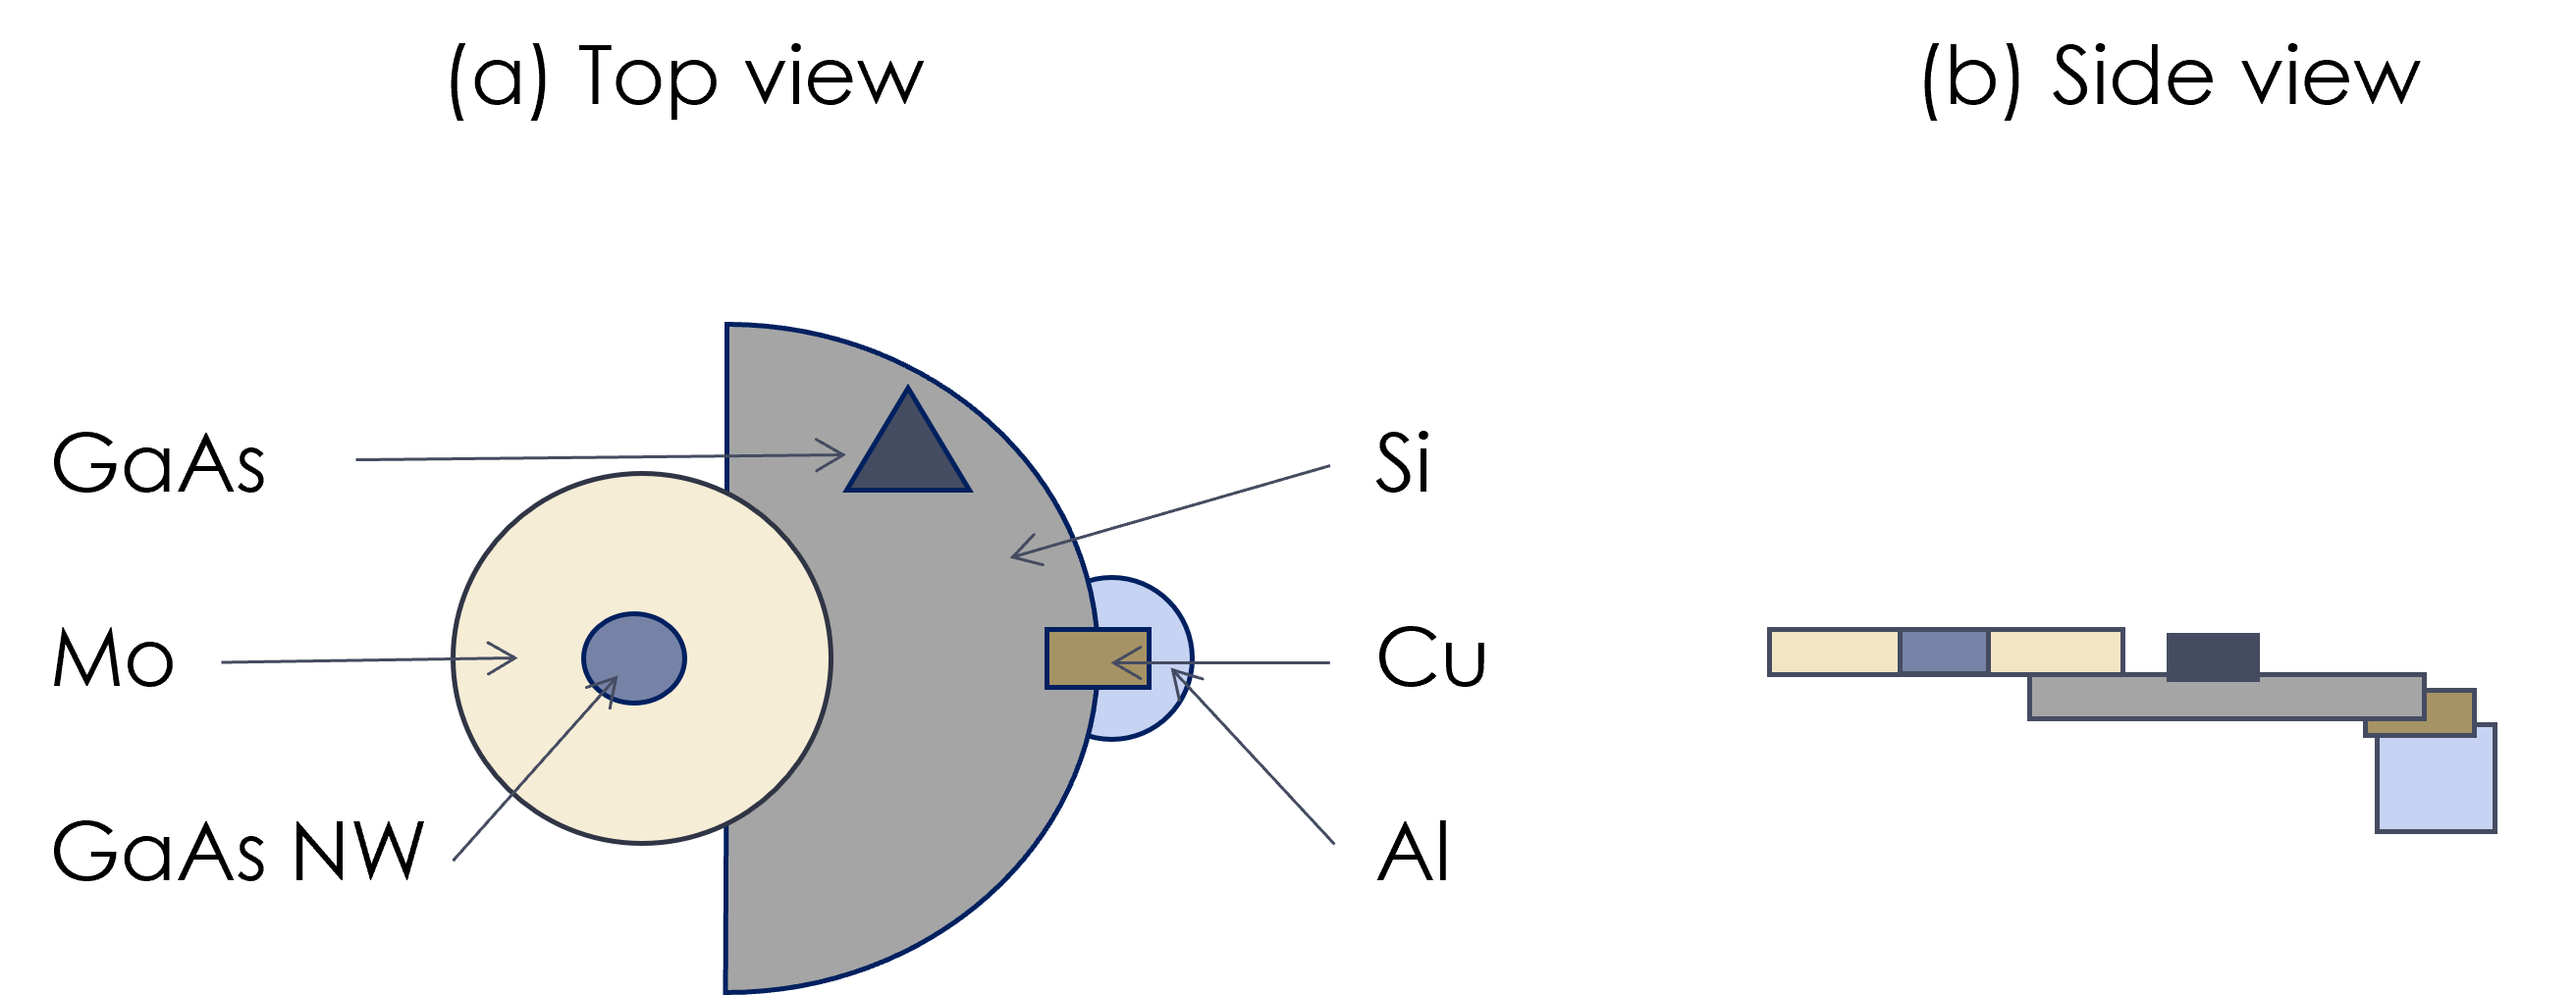
\includegraphics[width=0.7\textwidth]{../tex_prosjektoppgaven/figures/Materials-sample1.png}}
    \caption{
        The sample used for the EDS data collection in the SEM Apreo.
        (a) is top view and (b) is side view.
        GaAs is a piece of a GaAs wafer.
        Mo is a Mo disk.
        GaAs NW is the TEM grid of Mo with C film and GaAs nanowires.
        Si is the Si wafer.
        Cu is the Cu tape.
        Al is the Al FIB stub.
        Four spectra with different $V_{acc}$ was collected on the GaAs, Mo, Si, and GaAs NW.
        One spectrum was taken on the Cu tape and the Al FIB stub.
    }
    \label{fig:method:materials:sample1}
\end{figure}



%
%
\section{The microscope and the detector}
\label{sec:method:detector}
The data in this project was collected with the SEM Apreo from FEI with an Oxford EDX detector at NTNU NanoLab.
The detector is an EDX Oxford Xmax 80 mm2 Solid angle detector, with reported energy resolution of 127 eV (Cite: ntnu.norfab.no on the instrument).
The acceleration voltage, $V_{acc}$, can be set from 0.2 to 30 kV.
The beam current, $I_{beam}$, has a maximum value of 400 nA.
The SEM has an adjustable working distance.
The SEM is equipped with a BSE and a SE detector.

% my settings
The data collection was done on 5, 10, 15, and 30 kV.
The beam current was 0.2, 0.4, 0.8, or 1.6 nA, depending on the dead time of the detector, trying to get the dead time around 30\%.
All samples were collected on 2048 channels ranging from 0 to 20 keV.
Working distance was 10 mm.
Processing time was set to 5 and each spectrum was collected with 2 minutes time live.
Some spectra were stopped early due to high dead time and thus very long sampling.
At leas one SE picture was taken for each sampling area.

\ton{Is this enough to reproduce the data? I think so.}


%
%
\section{Analysis in AZtec}
\label{sec:method:aztec}
How to get the results from AZtec, what buttons and settings to use.
Which results AZtec gives: elements, concentrations, uncertainties, k-factors, etc.

%
%
\section{Extracting the data}
\label{sec:method:extracting}
The help from Mari and from Daniel.
What data I took out from AZtec.
Why I needed the k-factors from AZtec.


%
%
\section{Analysis in HyperSpy}
\label{sec:method:hspy}
What HyperSpy needs to do the analysis.
What functions I used in HyperSpy.
The different quantification methods in HyperSpy.
The results from HyperSpy: concentration, uncertainties

%
%
\section{Data treatment}
\label{sec:method:treatment}
In this project the data was also analyzed with new code, which is available on the GitHub.
The repository "eds-analysis"\footnote{\url{https://github.com/brynjarmorka/eds-analysis/}} contains the code developed throughout the semester, and the repository "eds-analysis-final"\footnote{\url{https://github.com/brynjarmorka/}} contains the final code.
\brynjar{Make the "eds-analysis-final" repository public.}
The code is written in Python and uses Jupyter notebooks.
NumPy is used for calculations, SciPy for fitting and peak finding, and Plotly for plotting \ton{do I to reference these packages?}.


\subsection{Calibration}
\label{sec:method:treatment:calibration}
A third repository, "spectroscopy-channel-calibration"\footnote{\url{https://github.com/brynjarmorka/spectroscopy-channel-calibration}}, was made specifically for calibration of spectra, which was used in the course "TFY4255 - Materials Physics" at NTNU, October 2022.
The calibration is done with a spectrum of known elements, where the user inputs the energy of the peaks.
The user further specifies the channel value of two peaks.
The energy of the peaks are available through HyperSpy, or can be set manually from e.g. the X-ray booklet.
The code makes a Gaussian fit to the two peaks, to find the true peak center.
A plot of the spectrum and the fit are shown, and the user can decide if the fit is good enough.
The code then calculates the dispersion, and the zero-offset.
In the end the code plots the spectrum with the calibration, and the user can decide if the calibration is good enough.
The same calibration is implemented in "eds-analysis-final", but without the plots and the user interaction.
\brynjar{Implement the sentence above.}



\subsection{Background subtraction}
\label{sec:method:treatment:background}
I subtracted the background from the spectra to see if the quantification would be better.
Linear background subtraction.
Sixth order polynomial background subtraction.
Additional subtraction?

\subsection{Area under the peaks}
\label{sec:method:treatment:area}
I calculated the area under the peaks to see if working on the raw data could help make the quantification better than AZtec and HyperSpy.


%
%
\section{Data from Mari?}
\label{sec:method:mar}
\ton{Do I need this? Is it to compare with my results? Or did you mean to use Maris code to get additional results?}
